

%% AAPT Physics Olympiad F=ma Questions
%%----------------------------------------


%% this section contains 60 problems


%% PhysicsOlympiad 2015
%%----------------------------------------
\element{aapt}{ %% Olympiad-A6
\begin{question}{Olympiad-2015-Q14}
    %%The following information applies to questions 14 and 15
    A \SI{3.0}{\meter} long massless rod is free to rotate horizontally about its center.
    Two \SI{5.0}{\kilo\gram} point objects are originally located at the ends of the rod;
        they are free to slide on the frictionless rod and are kept from flying off the rod by an inflexible massless rope that connects the two objects.
    Originally the system is rotating at \SI{4.0}{\radian\per\second};
        assume the system is completely frictionless;
        and ignore any concerns about instability of the system.
    %% Begin Question
    Calculate the original tension in the rope.
    \begin{multicols}{3}
    \begin{choices}
        \wrongchoice{\SI{60}{\newton}}
        \wrongchoice{\SI{106}{\newton}}
      \correctchoice{\SI{120}{\newton}}
        \wrongchoice{\SI{240}{\newton}}
        \wrongchoice{\SI{480}{\newton}}
    \end{choices}
    \end{multicols}
\end{question}
}

\element{aapt}{ %% Olympiad-A6
\begin{question}{Olympiad-2015-Q15}
    %%The following information applies to questions 14 and 15
    A \SI{3.0}{\meter} long massless rod is free to rotate horizontally about its center.
    Two \SI{5.0}{\kilo\gram} point objects are originally located at the ends of the rod;
        they are free to slide on the frictionless rod and are kept from flying off the rod by an inflexible massless rope that connects the two objects.
    Originally the system is rotating at \SI{4.0}{\radian\per\second};
        assume the system is completely frictionless;
        and ignore any concerns about instability of the system.
    %% Begin Question
    The rope is slowly tightened by a small massless motor attached to one of the objects.
    It is done in such a way as to pull the two objects closer to the center of the rotating rod.
    How much work is done by the motor in pulling the two objects from the ends of the rod until they are each \SI{0.5}{\meter} from the center of rotation?
    \begin{multicols}{3}
    \begin{choices}
        \wrongchoice{\SI{120}{\joule}}
        \wrongchoice{\SI{180}{\joule}}
        \wrongchoice{\SI{240}{\joule}}
      \correctchoice{\SI{1440}{\joule}}
        \wrongchoice{\SI{1620}{\joule}}
    \end{choices}
    \end{multicols}
\end{question}
}

\element{aapt}{ %% Olympiad-A6
\begin{question}{Olympiad-2015-Q17}
    A flywheel can rotate in order to store kinetic energy.
    The flywheel is a uniform disk made of a material with a density $\rho$ and tensile strength $\sigma$ (measured in Pascals---\si{\pascal}),
        a radius $r$, and a thickness $h$.
    The flywheel is rotating at the maximum possible angular velocity so that it does not break.
    Which of the following expression correctly gives the maximum kinetic energy per kilogram that can be stored in the flywheel?
    Assume that $\alpha$ is a dimensionless constant.
    \begin{multicols}{2}
    \begin{choices}
        \wrongchoice{$\alpha \sqrt{\dfrac{\rho \sigma}{4}}$}
        \wrongchoice{$\alpha h\sqrt{\dfrac{\rho\sigma}{r}}$}
        \wrongchoice{$\alpha \sqrt{\dfrac{h}{r}}\left(\dfrac{\sigma}{\rho}\right)^2$}
        \wrongchoice{$\alpha \left(\dfrac{h}{r}\right)\left(\dfrac{\sigma}{\rho}\right)$}
      \correctchoice{$\dfrac{\alpha\sigma}{\rho}$}
    \end{choices}
    \end{multicols}
\end{question}
}


%% PhysicsOlympiad 2014
%%----------------------------------------
\element{aapt}{ %% Olympiad-A6
\begin{question}{Olympiad-2014-Q01}
    A car turning to the right is traveling at constant speed in a circle.
    From the driver's perspective,
        the angular momentum vector about the center of the circle
        points $X$ and the acceleration vector of the car points $Y$ where
    \begin{choices}
        \wrongchoice{$X$ is left, $Y$ is left.}
        \wrongchoice{$X$ is forward, $Y$ is right.}
        \wrongchoice{$X$ is down, $Y$ is forward.}
        \wrongchoice{$X$ is left, $Y$ is right.}
      \correctchoice{$X$ is down, $Y$ is right.}
    \end{choices}
\end{question}
}

\element{aapt}{ %% Olympiad-A6
\begin{question}{Olympiad-2014-Q05}
    A unicyclist goes around a circular track of radius \SI{30}{\meter}
        at a (\emph{amazingly fast}!) constant speed of \SI{10}{\meter\per\second}.
    At what angle to the left (or right) of vertical must the unicyclist lean to avoid falling?
    Assume that the height of the unicyclist is much smaller than the radius of the track.
    \begin{multicols}{3}
    \begin{choices}
        \wrongchoice{\ang{9.46}}
        \wrongchoice{\ang{9.59}}
      \correctchoice{\ang{18.4}}
        \wrongchoice{\ang{19.5}}
        \wrongchoice{\ang{70.5}}
    \end{choices}
    \end{multicols}
\end{question}
}

\element{aapt}{ %% Olympiad-A6
\begin{question}{Olympiad-2014-Q07}
    A \SI{1.00}{\meter} long stick with uniform density is allowed
        to rotate about a point \SI{30.0}{\centi\meter} from its end.
    The stick is perfectly balanced when a \SI{50.0}{\gram}
        mass is placed on the stick \SI{20.0}{\centi\meter} from the same end.
    What is the mass of the stick?
    \begin{multicols}{3}
    \begin{choices}
        \wrongchoice{\SI{35.7}{\gram}}
        \wrongchoice{\SI{33.3}{\gram}}
      \correctchoice{\SI{25.0}{\gram}}
        \wrongchoice{\SI{17.5}{\gram}}
        \wrongchoice{\SI{14.3}{\gram}}
    \end{choices}
    \end{multicols}
\end{question}
}

\element{aapt}{ %% Olympiad-A6
\begin{question}{Olympiad-2014-Q10}
    A radio controlled car is attached to a stake in the ground by a \SI{3.00}{\meter}
        long piece of string, and is forced to move in a circular path.
    The car has an initial angular velocity of \SI{1.00}{\radian\per\second}
        and smoothly accelerates at a rate of \SI{4.00}{\radian\per\second\squared}.
    The string will break if the centripetal acceleration exceeds
        \SI{2.43e2}{\gram\per\second\squared}.
    How long can the car accelerate at this rate before the string breaks?
    \begin{multicols}{3}
    \begin{choices}
        \wrongchoice{\SI{0.25}{\second}}
        \wrongchoice{\SI{0.50}{\second}}
        \wrongchoice{\SI{1.00}{\second}}
        \wrongchoice{\SI{1.50}{\second}}
      \correctchoice{\SI{2.00}{\second}}
    \end{choices}
    \end{multicols}
\end{question}
}

\element{aapt}{ %% Olympiad-A6
\begin{question}{Olympiad-2014-Q14}
    A disk of moment of inertia $I$, mass $M$, and radius $R$ has a cord
        wrapped around it tightly as shown in the diagram.
    The disk is free to slide on its side as shown in the top down view.
    A constant force of $T$ is applied to the end of the cord and accelerates
        the disk along a frictionless surface.
    \begin{center}
    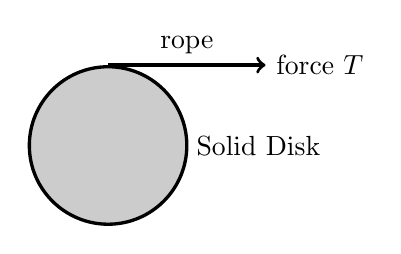
\begin{tikzpicture}
        \node[draw=black,very thick,fill=white!80!black,circle,minimum size=2cm] (A) at (0,0) {};
        \node[anchor=west,xshift=1cm] at (A) {Solid Disk};
        \draw[very thick,->] (A.north) -- ++ (0:2cm) node[pos=0.5,anchor=south] {rope} node[pos=1.0,anchor=west] {force $T$};
    \end{tikzpicture}
    \end{center}
    After the disk has accelerated some distance,
        determine the ratio of the translational $KE$ to total $KE$ of the disk,
    \begin{displaymath}
        \frac{KE_{translational}}{KE_{total}} =
    \end{displaymath}
    \begin{multicols}{3}
    \begin{choices}
        \wrongchoice{$\dfrac{1}{MR^2}$}
        \wrongchoice{$\dfrac{MR^2}{1}$}
        \wrongchoice{$\dfrac{1}{3MR^2}$}
      \correctchoice{$\dfrac{1}{MR^2+I}$}
        \wrongchoice{$\dfrac{MR^2}{MR^2+I}$}
    \end{choices}
    \end{multicols}
\end{question}
}

\element{aapt}{ %% Olympiad-A6
\begin{question}{Olympiad-2014-Q15}
    The maximum torque output from the engine of a new experimental car of mass $m$ is $\tau$.
    The maximum rotational speed of the engine is $\omega$.
    The engine is designed to provide a constant power output $P$.
    The engine is connected to the wheels via a perfect transmission
        that can smoothly trade torque for speed with no power loss.
    The wheels have a radius $R$,
        and the coefficient of static friction between the wheels and the road is $\mu$.
    %% Start Question
    What is the maximum sustained speed $v$ the car can drive up a \ang{30} incline?
    Assume no frictional losses and assume $\mu$ is large enough so that the tires do not slip.
    \begin{multicols}{2}
    \begin{choices}
      \correctchoice{$v=\dfrac{2P}{mg}$}
        \wrongchoice{$v=\dfrac{2P}{\sqrt{3}mg}$}
        \wrongchoice{$v=\dfrac{2P}{\mu mg}$}
        \wrongchoice{$v=\dfrac{\tau\omega}{mg}$}
        \wrongchoice{$v=\dfrac{\tau\omega}{\mu mg}$}
    \end{choices}
    \end{multicols}
\end{question}
}

\element{aapt}{ %% Olympiad-A6
\begin{question}{Olympiad-2014-Q20}
    A crew of scientists has built a new space station.
    The space station is shaped like a wheel of radius $R$,
        with essentially all its mass $M$ at the rim.
    When the crew arrives, the station will be set rotating at a rate that
        causes an object at the rim to have radial acceleration $g$, thereby simulating
    Earth's surface gravity.
    This is accomplished by two small rockets, each with thrust $T$ newtons,
        mounted on the station's rim.
    How long a time $t$ does one need to fire the rockets to achieve the desired condition?
    \begin{multicols}{2}
    \begin{choices}
        \wrongchoice{$t=\dfrac{\sqrt{g R^3} M}{2T}$}
      \correctchoice{$t=\dfrac{\sqrt{g R} M}{2T}$}
        \wrongchoice{$t=\dfrac{\sqrt{g R} M}{T}$}
        \wrongchoice{$t=\sqrt{\dfrac{g R}{\pi}}\dfrac{M}{T}$}
        \wrongchoice{$t=\dfrac{\sqrt{g R}M}{\pi T}$}
    \end{choices}
    \end{multicols}
\end{question}
}

\element{aapt}{ %% Olympiad-A6
\begin{question}{Olympiad-2014-Q21}
    Two pulleys (shown in figure) are made of the same metal with density $\rho$.
    Pulley $A$ is a uniform disk with radius $R$.
    Pulley $B$ is identical except a circle of $\frac{R}{2}$ is removed from the center.
    When two boxes $M=\alpha m$, where $\alpha>1$,
        are connected over the pulleys through a massless rope and move without slipping,
        what is the ratio between the accelerations in system $A$ and $B$?
    \begin{center}
    \begin{tikzpicture}
        \begin{scope}[xshift=+2cm]
            %% Labels
            \node[anchor=south]at (0,1em) {Pulley $B$};
            %% Ceiling
            \node[anchor=south,fill,pattern=north east lines,minimum width=3cm, minimum height=0.05cm] at (-0.5,0) {};
            \draw (-2,0) -- (1,0);
            %% Pulley
            \draw[fill=white!50!black] (0,-1) circle (0.75);
            \draw[fill=white] (0,-1) circle (0.38);
            \draw[fill=white!90!black] (-0.3,0) -- (-0.10,-1.1) arc(190:350:0.10) -- (0.3,0) --cycle;
            \draw[fill] (0,-1) circle (1.5pt);
            %% Masses
            \node[draw,fill=white!90!black,rectangle,rounded corners=1ex,minimum size=1cm,anchor=north] (A) at (-0.75,-3) {$m$};
            \node[draw,fill=white!90!black,rectangle,rounded corners=1ex,minimum size=1.414cm,anchor=north] (B) at (0.75,-2.5) {$M$};
            %% Rope
            \draw[thick] (A.north) -- (-0.75,-1.0) arc(180:0:0.75) -- (B.north);
        \end{scope}
        \begin{scope}[xshift=-2cm]
            %% Labels
            \node[anchor=south] at (0,1em) {Pulley $A$};
            %% Ceilin3737
            \node[anchor=south,fill,pattern=north east lines,minimum width=3cm, minimum height=0.05cm] at (+0.5,0) {};
            \draw (-1,0) -- (2,0);
            %% Pulley
            \draw[fill=white!50!black] (0,-1) circle (0.75);
            \draw[fill=white!90!black] (-0.3,0) -- (-0.2,-1.1) arc(190:350:0.2) -- (0.3,0) --cycle;
            \draw[fill] (0,-1) circle (1.5pt);
            %% Masses
            \node[draw,fill=white!90!black,rectangle,rounded corners=1ex,minimum size=1cm,anchor=north] (A) at (-0.75,-3) {$m$};
            \node[draw,fill=white!90!black,rectangle,rounded corners=1ex,minimum size=1.414cm,anchor=north] (B) at (0.75,-2.5) {$M$};
            %% Rope
            \draw[thick] (A.north) -- (-0.75,-1.0) arc(180:0:0.75) -- (B.north);
        \end{scope}
    \end{tikzpicture}
    \end{center}
    The mass of pulley $A$ is $M+m$.
    \begin{multicols}{2}
    \begin{choices}
      \correctchoice{$\dfrac{a_A}{a_B} = \dfrac{47}{48}$}
        \wrongchoice{$\dfrac{a_A}{a_B} = \dfrac{31}{32}$}
        \wrongchoice{$\dfrac{a_A}{a_B} = \dfrac{15}{16}$}
        \wrongchoice{$\dfrac{a_A}{a_B} = \dfrac{9}{16}$}
        \wrongchoice{$\dfrac{a_A}{a_B} = \dfrac{3}{4}$}
    \end{choices}
    \end{multicols}
\end{question}
}


%% PhysicsOlympiad 2013
%%----------------------------------------
\element{aapt}{ %% Olympiad-A6
\begin{question}{Olympiad-2013-Q04}
    The sign shown below consists of two uniform legs attached by a frictionless hinge.
    The coefficient of friction between the ground and the legs is $\mu$.
    Which of the following gives the maximum value of $\theta$ such that the sign will not collapse?
    \begin{center}
    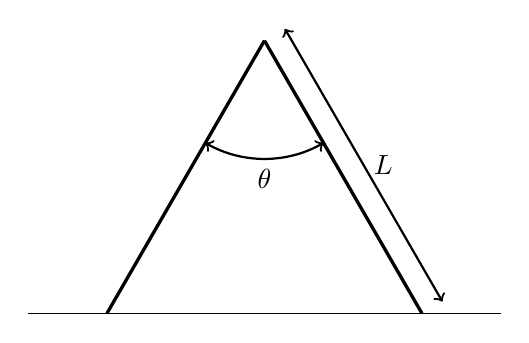
\begin{tikzpicture}
        %% Triangle
        \draw (-3,0) -- (3,0);
        \draw[very thick] (-2,0) -- ++ (60:4);
        \draw[very thick] (+2,0) -- ++ (120:4);
        %% Angle
        \draw[thick,<->] (-2,0) ++ (60:2.5) arc (240:300:1.5) node[pos=0.5,anchor=north] {$\theta$};
        %% Length
        \draw[thick,<->] (2,0) ++ (30:0.3) -- ++ (120:4) node[pos=0.5,anchor=west] {$L$};
    \end{tikzpicture}
    \end{center}
    \begin{multicols}{2}
    \begin{choices}
        \wrongchoice{$\sin\theta = 2\mu$}
        \wrongchoice{$\sin\dfrac{\theta}{2} = \dfrac{\mu}{2}$}
        \wrongchoice{$\tan\dfrac{\theta}{2} = \mu$}
        \wrongchoice{$\tan\theta = 2\mu$}
      \correctchoice{$\tan\dfrac{\theta}{2} = 2\mu$}
    \end{choices}
    \end{multicols}
\end{question}
}

\element{aapt}{ %% Olympiad-A6
\begin{question}{Olympiad-2013-Q10}
    Which of the following can be used to distinguish a solid ball
        from a hollow sphere of the same radius and mass?
    \begin{choices}
        \wrongchoice{Measurements of the orbit of a test mass around the object.}
      \correctchoice{Measurements of the time it takes the object to roll down an inclined plane.}
        \wrongchoice{Measurements of the tidal forces applied by the object to a liquid body.}
        \wrongchoice{Measurements of the behavior of the object as it floats in water.}
        \wrongchoice{Measurements of the force applied to the object by a uniform gravitational field.}
    \end{choices}
\end{question}
}

\element{aapt}{ %% Olympiad-A6
\begin{question}{Olympiad-2013-Q12}
    A spherical shell of mass $M$ and radius $R$ is completely filled with a frictionless fluid,
        also of mass $M$.
    It is released from rest,
        and then it rolls without slipping down an incline that makes an angle $theta$ with the horizontal.
    What will be the acceleration of the shell down the incline just after it is released?
    Assume the acceleration of free fall is $g$.
    The moment of inertia of a thin shell of radius $r$ and mass $m$ about the center of mass is $ =\frac{3}{2}mr^2$;
        the moment of inertia of a solid sphere of radius $r$ and mass $m$ about the center of mass is $I=\frac{2}{5} mr^2$.
    \begin{multicols}{2}
    \begin{choices}
        \wrongchoice{$a=g\sin\theta$}
      \correctchoice{$a=\dfrac{3g}{4}\sin\theta$}
        \wrongchoice{$a=\dfrac{g}{2}\sin\theta$}
        \wrongchoice{$a=\dfrac{3g}{8}\sin\theta$}
        \wrongchoice{$a=\dfrac{3g}{5}\sin\theta$}
    \end{choices}
    \end{multicols}
\end{question}
}


%% PhysicsOlympiad 2012
%%----------------------------------------
\element{aapt}{ %% Olympiad-A6
\begin{question}{Olympiad-2012-Q03}
    An equilateral triangle is sitting on an inclined plane.
    Friction is too high for it to slide under any circumstance,
        but if the plane is sloped enough it can ``topple'' down the hill.
    What angle incline is necessary for it to start toppling?
    \begin{choices}
        \wrongchoice{30 degrees}
        \wrongchoice{45 degrees}
      \correctchoice{60 degrees}
        \wrongchoice{It will topple at any angle more than zero}
        \wrongchoice{It can never topple if it cannot slide}
    \end{choices}
\end{question}
}

\element{aapt}{ %% Olympiad-A6
\begin{question}{Olympiad-2012-Q10}
    Four objects are placed at rest at the top of an inclined plane
        and allowed to roll without slipping to the bottom in the
        absence of rolling resistance and air resistance.
    \begin{itemize}
        \item Object $A$ is a solid brass ball of diameter $d$.
        \item Object $B$ is a solid brass ball of diameter $2d$.
        \item Object $C$ is a hollow brass sphere of diameter $d$.
        \item Object $D$ is a solid aluminum ball of diameter $d$. (Aluminum is less dense than brass.)
    \end{itemize}
    The balls are placed so that their centers of mass all travel the same distance.
    In each case, the time of motion $T$ is measured.
    Which of the following statements is correct?
    \begin{choices}
        \wrongchoice{$T_B > T_C > T_A = T_D$}
        \wrongchoice{$T_A = T_B = T_C > T_D$}
        \wrongchoice{$T_B > T_A = T_C = T_D$}
      \correctchoice{$T_C > T_A = T_B = T_D$}
        \wrongchoice{$T_A = T_B = T_C = T_D$}
    \end{choices}
\end{question}
}

\element{aapt}{ %% Olympiad-A6
\begin{question}{Olympiad-2012-Q12}
    A rigid hoop can rotate about the center.
    Two massless strings are attached to the hoop, one at $A$, the other at $B$.
    These strings are tied together at the center of the hoop at $O$,
        and a weight $G$ is suspended from that point.
    The strings have a fixed length, regardless of the tension,
        and the weight $G$ is only supported by the strings.
    Originally $OA$ is horizontal.
    \begin{center}
    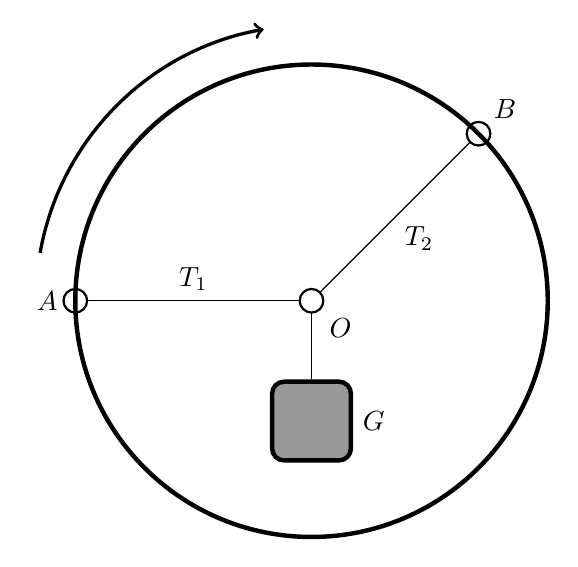
\begin{tikzpicture}
        \draw[ultra thick] (0,0) circle (3cm);
        \draw[thick] (0,0) circle (0.15cm);
        \node[anchor=north west] at (315:0.15cm) {$O$};
        %% 45 degree ring
        \draw[thick] (45:3) circle (0.15cm);
        \draw (45:0.15) -- (45:2.85) node[pos=0.5,anchor=north west] {$T_2$};
        \node[anchor=south west] at (45:3.1) {$B$};
        %% 180 degree ring
        \draw[thick] (180:3) circle (0.15cm);
        \draw (180:0.15cm) -- (180:2.85) node[pos=0.5,anchor=south] {$T_1$};
        \node[anchor=east] at (180:3.1) {$A$};
        %% Rotational direction
        \draw[very thick,->] (170:3.5) arc(170:100:3.5);
        %% handing mass
        \node[ultra thick,draw,fill=white!60!black,rounded corners=1ex,minimum size=1cm,anchor=north] (M) at (0,-1) {};
        \draw (M.north) -- (270:0.15cm);
        \node[anchor=west] at (M.east) {$G$};
    \end{tikzpicture}
    \end{center}
    Now, the outer hoop will start to slowly rotate \ang{90} clockwise
        until $OA$ will become vertical, while keeping the angle between
        the strings constant and keeping the object static.
    Which of the following statements about the tensions $T_1$ and $T_2$
        in the two strings is correct?
    \begin{choices}
        \wrongchoice{$T_1$ always decreases.}
        \wrongchoice{$T_1$ always increases.}
        \wrongchoice{$T_2$ always increases.}
      \correctchoice{$T_2$ will become zero at the end of the rotation.}
        \wrongchoice{$T_2$ first increases and then decreases.}
    \end{choices}
\end{question}
}

\element{aapt}{ %% Olympiad-A6
\begin{question}{Olympiad-2012-Q24}
    Three point masses $m$ are attached together by identical springs.
    When placed at rest on a horizontal surface the masses
        form a triangle with side length $l$.
    When the assembly is rotated about its center at angular velocity $\omega$,
        the masses form a triangle with side length $2l$.
    What is the spring constant $k$ of the springs?
    \begin{multicols}{3}
    \begin{choices}
        \wrongchoice{$2m\omega^2$}
        \wrongchoice{$\dfrac{2}{\sqrt{3}}m\omega^2$}
      \correctchoice{$\dfrac{2}{3}m\omega^2$}
        \wrongchoice{$\dfrac{1}{\sqrt{3}}m\omega^2$}
        \wrongchoice{$\dfrac{1}{3}m\omega^2$}
    \end{choices}
    \end{multicols}
\end{question}
}


%% PhysicsOlympiad 2011
%%----------------------------------------
\element{aapt}{ %% Olympiad-A6
\begin{question}{Olympiad-2011-Q07}
    An ice skater can rotate about a vertical axis with an
        angular velocity $\omega_0$ by holding her arms straight out.
    She can then pull in her arms close to her body so that her
        angular velocity changes to $2\omega_0$,
        without the application of any external torque.
    What is the ratio of her final rotational kinetic energy
        to her initial rotational kinetic energy?
    \begin{multicols}{3}
    \begin{choices}
        \wrongchoice{$\sqrt{2}$}
      \correctchoice{$2$}
        \wrongchoice{$2\sqrt{3}$}
        \wrongchoice{$4$}
        \wrongchoice{$8$}
    \end{choices}
    \end{multicols}
\end{question}
}

\element{aapt}{ %% Olympiad-A6
\begin{question}{Olympiad-2011-Q13}
    The apparatus in the diagram consists of a solid cylinder of radius
        \SI{1}{\centi\meter} attached at the center to two disks of radius \SI{2}{\centi\meter}.
    It is placed on a surface where it can roll, but will not slip.
    A thread is wound around the central cylinder.
    When the thread is pulled at the angle $\theta=\ang{90}$ to the horizontal (directly up),
        the apparatus rolls to the right.
    Which below is the largest value of $\theta$ for which it will not roll
        to the right when pulling on the thread?
    \begin{center}
        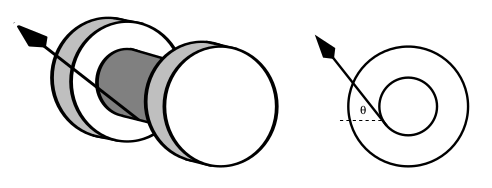
\includegraphics[keepaspectratio,scale=0.75]{Olympiad2011-Q13}
    \end{center}
    \begin{multicols}{2}
    \begin{choices}
        \wrongchoice{$\theta=\ang{15}$}
        \wrongchoice{$\theta=\ang{30}$}
        \wrongchoice{$\theta=\ang{45}$}
      \correctchoice{$\theta=\ang{60}$}
        \wrongchoice{None, the apparatus will always roll to the right}
    \end{choices}
    \end{multicols}
\end{question}
}

\element{aapt}{ %% Olympiad-A6
\begin{question}{Olympiad-2011-Q22}
    This graph depicts the torque output of a hypothetical gasoline engine
        as a function of rotation frequency.
    The engine is incapable of running outside of the graphed range.
    \begin{center}
    \begin{tikzpicture}
        \begin{axis}[
            clip=false,
            axis y line=left,
            axis x line=bottom,
            axis line style={->},
            xlabel={Engine Revolutions per Minute},
            xtick={0,1000,2000},
            minor x tick num=3,
            ylabel={Output Torque},
            y unit=\si{\newton\per\meter},
            ytick={0,10,20,30},
            minor y tick num=1,
            grid=major,
            xmin=0,ymax=35,
            ymin=0,xmax=2500,
            width=0.95\columnwidth,
            height=0.618\columnwidth,
        ]
        \addplot[very thick,smooth,mark=\empty] plot coordinates { (250,12) (750,16) (1500,31) (2000,22) (2250,5) };
        \draw[fill] (axis cs:250,12) circle (1.5pt) node[anchor=south] {$I$};
        \draw[fill] (axis cs:1500,31) circle (1.5pt) node[anchor=south] {$II$};
        \draw[fill] (axis cs:2250,5) circle (1.5pt) node[anchor=south west] {$III$};
        \end{axis}
    \end{tikzpicture}
    \end{center}
    At what engine RPM (revolutions per minute) does the engine produce maximum power?
    \begin{choices}[o]
        \wrongchoice{I}
        \wrongchoice{At some point between I and II}
        \wrongchoice{II}
      \correctchoice{At some point between II and III}
        \wrongchoice{III}
    \end{choices}
\end{question}
}

\element{aapt}{ %% Olympiad-A6
\begin{question}{Olympiad-2011-Q24}
    A turntable is supported on a Teflon ring of inner radius $R$ and outer radius $R+\delta$ where $\delta\ll R$, as shown in the diagram.
    To rotate the turntable at a constant rate, power must be supplied to overcome friction.
    The manufacturer of the turntable wishes to reduce the power required without changing the rotation rate,
        the weight of the turntable, or the coefficient of friction of the Teflon surface.
    Engineers propose two solutions: increasing the width of the bearing (increasing $\delta$),
        or increasing the radius (increasing $R$).
    What are the effects of these proposed changes?
    \begin{center}
    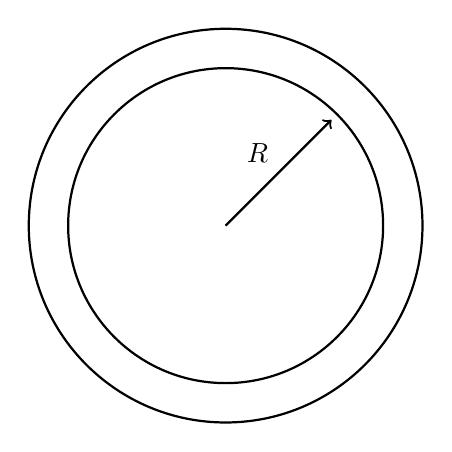
\begin{tikzpicture}
        \draw[thick] (0,0) circle (2cm);
        \draw[thick] (0,0) circle (2.5cm);
        \draw[thick,->] (0,0) -- ++(45:1.9cm) node[pos=0.5,anchor=south east] {$R$};
    \end{tikzpicture}
    \end{center}
    \begin{choices}
      \correctchoice{Increasing $\delta$ has no significant effect on the required power;
            increasing $R$ increases the required power.}
        \wrongchoice{Increasing $\delta$ has no significant effect on the required power;
            increasing $R$ decreases the required power.}
        \wrongchoice{Increasing $\delta$ increases the required power;
            increasing $R$ has no significant effect on the required power.}
        \wrongchoice{Increasing $\delta$ decreases the required power;
            increasing $R$ has no significant effect on the required power.}
        \wrongchoice{Neither change has a significant effect on the required power.}
    \end{choices}
\end{question}
}

\element{aapt}{ %% Olympiad-A6
\begin{question}{Olympiad-2011-Q25}
    A hollow cylinder with a very thin wall (like a toilet paper tube) and a block are placed at rest at the top of a plane with inclination $\theta$ above the horizontal.
    The cylinder rolls down the plane without slipping and the block slides down the plane;
        it is found that both objects reach the bottom of the plane simultaneously.
    What is the coefficient of kinetic friction between the block and the plane?
    \begin{multicols}{3}
    \begin{choices}
        \wrongchoice{zero}
        \wrongchoice{$\dfrac{1}{3}\tan\theta$}
      \correctchoice{$\dfrac{1}{2}\tan\theta$}
        \wrongchoice{$\dfrac{2}{3}\tan\theta$}
        \wrongchoice{$\tan\theta$}
    \end{choices}
    \end{multicols}
\end{question}
}


%% PhysicsOlympiad 2010
%%----------------------------------------
\element{aapt}{ %% Olympiad-A6
\begin{question}{Olympiad-2010-Q07}
    Harry Potter is sitting \SI{2.0}{\meter} from the center of a merry-go-round
        when Draco Malfoy casts a spell that glues Harry in place and then makes
        the merry-go-round start spinning on its axis.
    Harry has a mass of \SI{50.0}{\kilo\gram} and can withstand $\num{5.0}g's$
        of acceleration before passing out.
    What is the magnitude of Harry's angular momentum when he passes out?
    \begin{multicols}{2}
    \begin{choices}
        \wrongchoice{\SI{200}{\kilo\gram\meter\squared\per\second}}
        \wrongchoice{\SI{330}{\kilo\gram\meter\squared\per\second}}
        \wrongchoice{\SI{660}{\kilo\gram\meter\squared\per\second}}
      \correctchoice{\SI{1000}{\kilo\gram\meter\squared\per\second}}
        \wrongchoice{\SI{2200}{\kilo\gram\meter\squared\per\second}}
    \end{choices}
    \end{multicols}
\end{question}
}


%% PhysicsOlympiad 2009
%%----------------------------------------
\newcommand{\olympiadTwentyZeroNineQEight}{
\begin{tikzpicture}
    \begin{axis}[
        axis y line=left,
        axis x line=middle,
        axis line style={->},
        xlabel={time},
        x unit=\si{\second},
        xtick={0,1,2,3},
        minor x tick num=1,
        ylabel={angular velocity},
        y unit=\si{\radian\per\second},
        ytick={-2,0,2,4},
        minor x tick num=1,
        grid=major,
        xmin=0,xmax=3.3,
        ymin=-2.5,ymax=4.5,
        width=0.8\columnwidth,
        height=0.5\columnwidth,
    ]
    \addplot[line width=1pt,domain=0:3]{4 - 2*x};
    \end{axis}
\end{tikzpicture}
}

\element{aapt}{ %% Olympiad-A6
\begin{question}{Olympiad-2009-Q08}
    A flat disk rotates about an axis perpendicular to the plane of the
        disk and through the center of the disk with an angular velocity
        as shown in the graph below.
    \begin{center}
        \olympiadTwentyZeroNineQEight
    \end{center}
    Determine the angular acceleration of the disk when $t=\SI{2.0}{\second}$.
    \begin{multicols}{3}
    \begin{choices}
        \wrongchoice{\SI{-12}{\radian\per\second\squared}}
        \wrongchoice{\SI{-8}{\radian\per\second\squared}}
        \wrongchoice{\SI{-4}{\radian\per\second\squared}}
      \correctchoice{\SI{-2}{\radian\per\second\squared}}
        \wrongchoice{\SI{0}{\radian\per\second\squared}}
    \end{choices}
    \end{multicols}
\end{question}
}

\element{aapt}{ %% Olympiad-A6
\begin{question}{Olympiad-2009-Q09}
    A flat disk rotates about an axis perpendicular to the plane of the
        disk and through the center of the disk with an angular velocity
        as shown in the graph below.
    \begin{center}
        \olympiadTwentyZeroNineQEight
    \end{center}
    Through what net angle does the disk turn during the 3 seconds?
    \begin{multicols}{3}
    \begin{choices}
        \wrongchoice{\SI{9}{\radian}}
        \wrongchoice{\SI{8}{\radian}}
        \wrongchoice{\SI{6}{\radian}}
        \wrongchoice{\SI{4}{\radian}}
      \correctchoice{\SI{3}{\radian}}
    \end{choices}
    \end{multicols}
\end{question}
}

\element{aapt}{ %% Olympiad-A6
\begin{question}{Olympiad-2009-Q13}
    Lucy (mass \SI{33.1}{\kilo\gram}), Henry (mass \SI{63.7}{\kilo\gram}),
        and Mary (mass \SI{24.3}{\kilo\gram}) sit on a lightweight seesaw
        at evenly spaced \SI{2.74}{\meter} intervals
        (in the order in which they are listed; Henry is between Lucy and Mary)
        so that the seesaw balances.
    Who exerts the most torque (in terms of magnitude) on the seesaw?
    Ignore the mass of the seesaw.
    \begin{choices}
        \wrongchoice{Henry}
      \correctchoice{Lucy}
        \wrongchoice{Mary}
        \wrongchoice{They all exert the same torque.}
        \wrongchoice{There is not enough information to answer the question.}
    \end{choices}
\end{question}
}

\element{aapt}{ %% Olympiad-A6
\begin{question}{Olympiad-2009-Q24}
    A uniform rectangular wood block of mass $M$,
        with length $b$ and height $a$, rests on an incline as shown.
    The incline and the wood block have a coefficient of static friction, $\mu_s$.
    The incline is moved upwards from an angle of zero through an angle $\theta$.
    At some critical angle the block will either tip over or slip down the plane.
    \begin{center}
    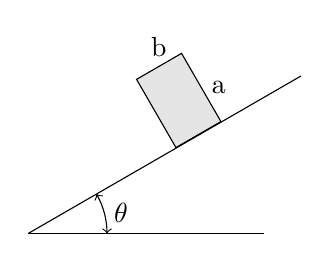
\begin{tikzpicture}
        %% surface
        \draw (0,0) -- (3,0);
        \draw (0,0) -- (30:4);
        %% block
        \node[draw,fill=white!90!black,rectangle,minimum height=1.00cm,minimum width=0.66cm,anchor=south,rotate=30] (M) at (30:2.5) {};
        \node[anchor=west] at (M.east) {a};
        \node[anchor=south] at (M.north) {b};
        %% angle
        \draw[<->] (0:1) arc (0:30:1) node[anchor=west,pos=0.5] {$\theta$};
    \end{tikzpicture}
    \end{center}
    Determine the relationship between $a$, $b$,
        and $\mu_s$ such that the block will tip over (and not slip) at the critical angle.
    The box is rectangular, and $a\neq b$.
    \begin{multicols}{2}
    \begin{choices}
        \wrongchoice{$\mu_s > \dfrac{a}{b}$}
        \wrongchoice{$\mu_s > 1 − \dfrac{a}{b}$}
      \correctchoice{$\mu_s > \dfrac{b}{a}$}
        \wrongchoice{$\mu_s < \dfrac{a}{b}$}
        \wrongchoice{$\mu_s < \dfrac{1}{b} − 1$}
    \end{choices}
    \end{multicols}
\end{question}
}


%% PhysicsOlympiad 2008
%%----------------------------------------
\element{aapt}{ %% Olympiad-A6
\begin{question}{Olympiad-2008-Q12}
    A uniform disk rotates at a fixed angular velocity on an axis through
        its center normal to the plane of the disk, and has kinetic energy $E$.
    If the same disk rotates at the same angular velocity about an axis
        on the edge of the disk (still normal to the plane of the disk),
        what is its kinetic energy?
    \begin{multicols}{3}
    \begin{choices}
        \wrongchoice{$\dfrac{1}{2}E$}
        \wrongchoice{$\dfrac{3}{2}E$}
        \wrongchoice{$2E$}
      \correctchoice{$3E$}
        \wrongchoice{$4E$}
    \end{choices}
    \end{multicols}
\end{question}
}

\element{aapt}{ %% Olympiad-A6
\begin{question}{Olympiad-2008-Q14}
    A spaceborne energy storage device consists of two equal masses connected
        by a tether and rotating about their center of mass.
    Additional energy is stored by reeling in the tether;
        no external forces are applied.
    Initially the device has kinetic energy $E$ and rotates at angular velocity $\omega$.
    Energy is added until the device rotates at angular velocity $2\omega$.
    What is the new kinetic energy of the device?
    \begin{multicols}{3}
    \begin{choices}
        \wrongchoice{$\sqrt{2}E$}
      \correctchoice{$2E$}
        \wrongchoice{$2\sqrt{2}E$}
        \wrongchoice{$4E$}
        \wrongchoice{$8E$}
    \end{choices}
    \end{multicols}
\end{question}
}

\element{aapt}{ %% Olympiad-A6
\begin{question}{Olympiad-2008-Q18}
    A uniform circular ring of radius $R$ is fixed in place.
    A particle is placed on the axis of the ring at a distance much greater
        than $R$ and allowed to fall towards the ring under the influence of the ring’s gravity.
    The particle achieves a maximum speed $v$.
    The ring is replaced with one of the same (linear) mass density but radius $2R$,
        and the experiment is repeated.
    What is the new maximum speed of the particle?
    \begin{multicols}{3}
    \begin{choices}
        \wrongchoice{$\dfrac{1}{2}v$}
        \wrongchoice{$\dfrac{1}{\sqrt{2}}v$}
      \correctchoice{$v$}
        \wrongchoice{$\sqrt{2}v$}
        \wrongchoice{$2v$}
    \end{choices}
    \end{multicols}
\end{question}
}



%% PhysicsOlympiad 2007
%%----------------------------------------
\element{aapt}{ %% Olympiad-A6
\begin{question}{Olympiad-2007-Q10}
    Two wheels with fixed hubs, each having a mass of \SI{1}{\kilo\gram},
        start from rest, and forces are applied as shown.
    \begin{center}
    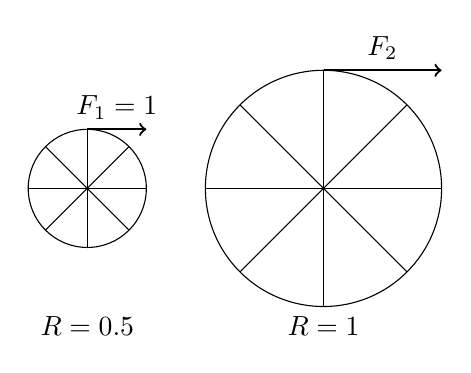
\begin{tikzpicture}
        %% Large
        \begin{scope}[xshift=+2cm,scale=0.75]
            %% Circle with spokes
            \draw (0,0) circle (2cm);
            \foreach \x in {45,90,...,360} {
                \draw (0,0) -- (\x:2cm);
            }
            %% Torquing force
            \draw[thick,->] (0,2) -- ++(0:2cm) node[pos=0.5,anchor=south] {$F_2$};
            %% Labels
            \node[anchor=north] at (0,-2) {$R=\SI{1}{\meter}$};
        \end{scope}
        %% Small
        \begin{scope}[xshift=-1cm,scale=0.75]
            %% Circle with spokes
            \draw (0,0) circle (1cm);
            \foreach \x in {45,90,...,360} {
                \draw (0,0) -- (\x:1cm);
            }
            %% Torquing force
            \draw[thick,->] (0,1) -- ++(0:1cm) node[pos=0.5,anchor=south] {$F_1=\SI{1}{\newton}$};
            %% Labels
            \node[anchor=north] at (0,-2) {$R=\SI{0.5}{\meter}$};
        \end{scope}
    \end{tikzpicture}
    \end{center}
    Assume the hubs and spokes are massless,
        so that the rotational inertia is $I = mR^2$.
    In order to impart identical angular accelerations
        about their respective hubs, how large must $F_2$ be?
    \begin{multicols}{3}
    \begin{choices}
        \wrongchoice{\SI{0.25}{\newton}}
        \wrongchoice{\SI{0.5}{\newton}}
        \wrongchoice{\SI{1}{\newton}}
      \correctchoice{\SI{2}{\newton}}
        \wrongchoice{\SI{4}{\newton}}
    \end{choices}
    \end{multicols}
\end{question}
}

\element{aapt}{ %% Olympiad-A6
\begin{question}{Olympiad-2007-Q21}
    If the rotational inertia of a sphere about an axis through the
        center of the sphere is $I$, what is the rotational inertia
        of another sphere that has the same density, but has twice the radius?
    \begin{multicols}{3}
    \begin{choices}
        \wrongchoice{$2 I$}
        \wrongchoice{$4 I$}
        \wrongchoice{$8 I$}
        \wrongchoice{$16 I$}
      \correctchoice{$32 I$}
    \end{choices}
    \end{multicols}
\end{question}
}

\element{aapt}{ %% Olympiad-A6
\begin{question}{Olympiad-2007-Q15}
    A uniform disk ($I=\frac{1}{2} MR^2$) of mass \SI{8.0}{\kilo\gram}
        can rotate without friction on a fixed axis.
    \begin{center}
    \begin{tikzpicture}
        %% Ceiling
        \node[anchor=south,fill,pattern=north east lines,minimum width=4cm, minimum height=0.05cm] at (0,0) {};
        \draw (-2,0) -- (2,0);
        %% Pulley
        \draw (0,-1) circle (0.75);
        \draw[fill=white!90!black] (-0.3,0) -- (-0.2,-1.1) arc(190:350:0.2) -- (0.3,0) --cycle;
        \draw[fill] (0,-1) circle (1.5pt);
        %% Masses
        \node[draw,fill=white!90!black,rectangle,rounded corners=1ex,minimum size=1.414cm,anchor=north] (M) at (0.75,-3) {\SI{3.0}{\kilo\gram}};
        %% Rope
        \draw[thick] (M.north) -- (0.75,-1.0);
    \end{tikzpicture}
    \end{center}
    A string is wrapped around its circumference and is attached
        to a \SI{6.0}{\kilo\gram} mass.
    The string does not slip.
    What is the tension in the cord while the mass is falling?
    \begin{multicols}{3}
    \begin{choices}
        \wrongchoice{\SI{20.0}{\newton}}
      \correctchoice{\SI{24.0}{\newton}}
        \wrongchoice{\SI{34.3}{\newton}}
        \wrongchoice{\SI{60.0}{\newton}}
        \wrongchoice{\SI{80.0}{\newton}}
    \end{choices}
    \end{multicols}
\end{question}
}

\element{aapt}{ %% Olympiad-A6
\begin{question}{Olympiad-2007-Q31}
    A thin, uniform rod has mass $m$ and length $L$.
    Let the acceleration due to gravity be $g$.
    Let the rotational inertia of the rod about its center be $md^2$.
    %% Start Question
    Find the ratio $\frac{L}{d}$.
    \begin{multicols}{2}
    \begin{choices}
        \wrongchoice{$3\sqrt{2}$}
        \wrongchoice{$3$}
        \wrongchoice{$12$}
      \correctchoice{$2\sqrt{3}$}
        \wrongchoice{none of the provided}
    \end{choices}
    \end{multicols}
\end{question}
}


%% PhysicsOlympiad 2004
%%----------------------------------------
\element{aapt}{ %% Olympiad-A6
\begin{question}{Olympiad-2004-Q14}
    A heavy, uniform metal disk starts from rest and rolls down an incline plane with height $h$.
    \begin{center}
    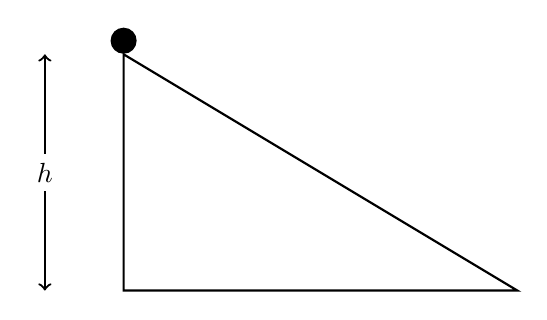
\begin{tikzpicture}
        %% Block and ball
        \draw[thick] (0,3) -- (0,0) -- (5,0) -- cycle;
        \node[circle,fill,anchor=south] at (0,3) {};
        %% height
        \draw[thick,<->] (-1,0) -- (-1,3) node[pos=0.5,anchor=center,fill=white] {$h$};
    \end{tikzpicture}
    \end{center}
    Assume there is not mechanical energy lost to friction and that air resistance is negligible.
    When the disk reaches the bottom of the plane its velocity would be:
    \begin{multicols}{3}
    \begin{choices}
        \wrongchoice{$\sqrt{2hg}$}
      \correctchoice{$\sqrt{\dfrac{4hg}{3}}$}
        \wrongchoice{$\left(2gh\right)^2$}
        \wrongchoice{$\left(3gh\right)^2$}
        \wrongchoice{$\dfrac{4gh}{3}$}
    \end{choices}
    \end{multicols}
\end{question}
}


%% PhysicsOlympiad 2003
%%----------------------------------------
\element{aapt}{ %% Olympiad-A6
\begin{question}{Olympiad-2003-Q09}
    A uniform ladder in static equilibrium leans against a frictionless wall.
    \begin{center}
    \begin{tikzpicture}
        %% Wall
        \node[anchor=west,fill,pattern=north east lines,minimum width=0.1cm, minimum height=3cm] at (0,1.5) {};
        \draw (0,0) -- (0,3);
        %% Floor
        \node[anchor=north,fill,pattern=north east lines,minimum width=4.2cm, minimum height=0.1cm] at (-1.9,0) {};
        \draw (0,0) -- (-4,0);
        %% Ladder
        \draw[line width=3pt] (0,2.12) -- (-3,0) node[pos=0.5,anchor=south east] {ladder};
        %% angle
        \draw[<->] (-2,0) arc (0:30:1) node[pos=0.5,anchor=west] {\ang{30}};
    \end{tikzpicture}
    \end{center}
    The ladder has length $L$ and mass $M$.
    Given that the angle between the ladder and floor is \ang{30} degrees,
        what would be the value of the coefficient of static friction ($\mu_s$) between the ladder and the ground?
    \begin{multicols}{2}
    \begin{choices}
        \wrongchoice{$\mu_s \geq \dfrac{1}{\sqrt{3}}$}
        \wrongchoice{$\mu_s \geq \dfrac{2}{\sqrt{3}}$}
      \correctchoice{$\mu_s \geq \dfrac{\sqrt{3}}{2}$}
        \wrongchoice{$\mu_s \geq \dfrac{1}{2}$}
        \wrongchoice{$\mu_s \geq \sqrt{3}$}
    \end{choices}
    \end{multicols}
\end{question}
}

\element{aapt}{ %% Olympiad-A6
\begin{question}{Olympiad-2003-Q13}
    %% THE NEXT TWO QUESTIONS REFER TO THE FOLLOWING SCENARIO
    A figure skater has a moment of inertia of \SI{4.0}{\kilo\gram\meter\squared} with her arms outstretched.
    If she begins a spin at \SI{3.0}{\radian\per\second} with her arms outstretched and then brings her arms in tight to her body,
    her rate of spin increases to \SI{7.0}{\radian\per\second} in \SI{2.5}{\second}.
    You may ignore friction and air resistance.
    %% start question
    As the skater brings her arms in tight to her body,
        what torque is applied to increase her spin.
    \begin{multicols}{2}
    \begin{choices}
        \wrongchoice{\SI{2.7}{\newton\meter}}
        \wrongchoice{\SI{4.0}{\newton\meter}}
        \wrongchoice{\SI{5.3}{\newton\meter}}
        \wrongchoice{\SI{9.3}{\newton\meter}}
      \correctchoice{no torque is applied to increase her spin}
    \end{choices}
    \end{multicols}
\end{question}
}

\element{aapt}{ %% Olympiad-A6
\begin{question}{Olympiad-2003-Q14}
    %% THE NEXT TWO QUESTIONS REFER TO THE FOLLOWING SCENARIO
    A figure skater has a moment of inertia of \SI{4.0}{\kilo\gram\meter\squared} with her arms outstretched.
    If she begins a spin at \SI{3.0}{\radian\per\second} with her arms outstretched and then brings her arms in tight to her body,
    her rate of spin increases to \SI{7.0}{\radian\per\second} in \SI{2.5}{\second}.
    You may ignore friction and air resistance.
    %% start question
    What is the moment of inertia of the skater with her arms tight to her body?
    \begin{multicols}{2}
    \begin{choices}
        \wrongchoice{\SI{0.73}{\kilo\gram\meter\squared}}
      \correctchoice{\SI{1.7}{\kilo\gram\meter\squared}}
        \wrongchoice{\SI{2.8}{\kilo\gram\meter\squared}}
        \wrongchoice{\SI{7.5}{\kilo\gram\meter\squared}}
        \wrongchoice{\SI{9.4}{\kilo\gram\meter\squared}}
    \end{choices}
    \end{multicols}
\end{question}
}


%% PhysicsOlympiad 2000
%%----------------------------------------
\element{aapt}{ %% Olympiad-A6
\begin{question}{olympiad-2000-q04}
    An Olympic ice skater starts a slow spin on her ice skates.
    As she brings her arm and free leg closer to her axis of rotation,
        she spins faster.
    Which of the following statements must he true?
    \begin{choices}
      \correctchoice{Angular momentum remains constant but angular kinetic energy increases.}
        \wrongchoice{Angular momentum increases but angular kinetic energy remains the same.}
        \wrongchoice{Both angular momentum and angular kinetic energy increase.}
        \wrongchoice{Both angular momentum and angular kinetic energy remain the same.}
        \wrongchoice{All of the provided might he true depending on the type of spin.}
    \end{choices}
\end{question}
}

\element{aapt}{ %% Olympiad-A6
\begin{question}{olympiad-2000-q15}
    A wheel starts from rest and angularly accelerates with a constant angular acceleration.
    After a time $t$, the wheel completes its first revolution,
        about how long will it take to complete its second revolution?
    \begin{multicols}{3}
    \begin{choices}
      \correctchoice{$0.4 t$}
        \wrongchoice{$1.0 t$}
        \wrongchoice{$1.4 t$}
        \wrongchoice{$1.7 t$}
        \wrongchoice{$2.0 t$}
    \end{choices}
    \end{multicols}
\end{question}
}


%% PhysicsOlympiad 1999
%%----------------------------------------
\element{aapt}{ %% Olympiad-A6
\begin{question}{olympiad-1999-q14}
    A thin ring of mass $m$ and radius $r$ rolls across the floor with a velocity $v$.
    Which of the following would be the best estimate of the ring's total kinetic energy as it rolls across the floor?
    \begin{multicols}{2}
    \begin{choices}
      \correctchoice{$mv^2$}
        \wrongchoice{$\dfrac{1}{2} mv^2$}
        \wrongchoice{$\dfrac{1}{4} mv^2$}
        \wrongchoice{$\dfrac{1}{2} mv^2 + \dfrac{mv^2}{r}$}
        \wrongchoice{$\dfrac{1}{2} mv^2 + \dfrac{mr^2}{t^2}$}
    \end{choices}
    \end{multicols}
\end{question}
}


%% PhysicsOlympiad 1998
%%----------------------------------------
\element{aapt}{ %% Olympiad-A6
\begin{question}{olympiad-1998-q09}
    A large spool of rope lies on the ground in the diagram below.
    \begin{center}
    \begin{tikzpicture}
        %% Ground
        \draw (-2,0) -- (+4,0);
        \node[anchor=north,fill,pattern=north east lines,minimum width=6cm, minimum height=0.05cm] at (1,0) {};
        %% Spool
        \draw[thick] (0,2) circle (2cm);
        %% Rope
        \draw[thick,->] (0,4) -- ++(0:4) node[anchor=north east] {$X$};
    \end{tikzpicture}
    \end{center}
    The end, labeled $X$, is pulled a distance $S$ in the horizontal direction.
    The spool rolls without slipping.
    The distance the spool’s center of mass moves is:
    \begin{multicols}{3}
    \begin{choices}
        \wrongchoice{$2S$}
        \wrongchoice{$S$}
      \correctchoice{$\dfrac{S}{2}$}
        \wrongchoice{$\dfrac{S}{3}$}
        \wrongchoice{$\dfrac{S}{4}$}
    \end{choices}
    \end{multicols}
\end{question}
}

\element{aapt}{ %% Olympiad-A6
\begin{question}{olympiad-1998-q15}
    Three identical objects of mass $M$ are fastened to a massless rod of length $L$ as shown.
    \begin{center}
    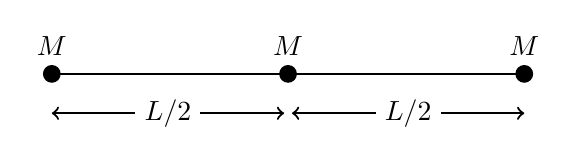
\begin{tikzpicture}
        %% three masses
        \draw[fill] (-3,0) circle (3pt) node[anchor=south,yshift=3pt] {$M$};
        \draw[fill] (+3,0) circle (3pt) node[anchor=south,yshift=3pt] {$M$};
        \draw[fill] (+0,0) circle (3pt) node[anchor=south,yshift=3pt] {$M$};
        %% connect
        \draw[thick] (-3,0) -- (3,0);
        %% labels
        \draw[thick,<->] (-3,-0.5) -- (-0.05,-0.5) node[pos=0.5,anchor=center,fill=white] {$L/2$};
        \draw[thick,<->] (+3,-0.5) -- (+0.05,-0.5) node[pos=0.5,anchor=center,fill=white] {$L/2$};
    \end{tikzpicture}
    \end{center}
    The array rotates about the center of the rod.
    Its rotational inertia is
    \begin{multicols}{3}
    \begin{choices}
      \correctchoice{$\dfrac{1}{2} ML^2$}
        \wrongchoice{$ML^2$}
        \wrongchoice{$\dfrac{5}{4} ML^2$}
        \wrongchoice{$\dfrac{3}{2} ML^2$}
        \wrongchoice{$3 ML^2$}
    \end{choices}
    \end{multicols}
\end{question}
}

\element{aapt}{ %% Olympiad-A6
\begin{question}{olympiad-1998-q17}
    Two identical bricks of length $L$ are piled one on top of the other on a table.
    %See the diagram to the right.
    \begin{center}
    \begin{tikzpicture}
        \draw (-4,0) -- (0,0) -- (0,-2);
        %% Blocks
        \node[draw,minimum width=2cm,minimum height=1cm,anchor=south] (A) at (-0.7,0) {};
        \node[draw,minimum width=2cm,minimum height=1cm,anchor=south,xshift=0.3cm] (B) at (A.north) {};
        %% labels
        \draw[thick,<->] (B.north west) ++(90:0.5) -- ++(0:2cm) node[pos=0.5,anchor=center,fill=white] {$L$};
        %% distance
        \draw[dashed] (B.south east) -- ++(270:2);
        \draw[thick,<-] (0,-0.5) -- ++(180:1);
        \draw[thick,<-] (0.6,-0.5) -- ++(0:1);
        \node[anchor=center] at (0.3,-0.5) {$S$};
    \end{tikzpicture}
    \end{center}
    What is the maximum distance $S$ the top brick can overlap the table with the system still balanced?
    \begin{multicols}{3}
    \begin{choices}
        \wrongchoice{$\dfrac{1}{2} L$}
        \wrongchoice{$\dfrac{2}{3} L$}
      \correctchoice{$\dfrac{3}{4} L$}
        \wrongchoice{$\dfrac{7}{8} L$}
        \wrongchoice{$ L$}
    \end{choices}
    \end{multicols}
\end{question}
}


%% PhysicsOlympiad 1997
%%----------------------------------------
\element{aapt}{ %% Olympiad-A6
\begin{question}{olympiad-1997-q08}
    A point object of mass $2m$ is attached to one end of a rigid rod of negligible mass and length $L$.
    The rod is initially at rest but free to rotate about a fixed axis perpendicular to the rod and passing through its other end.
    \begin{center}
    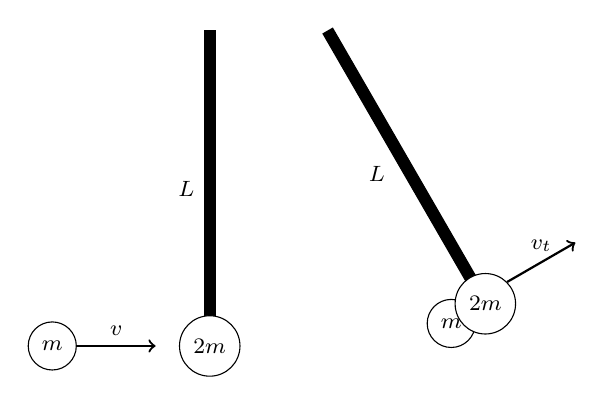
\begin{tikzpicture}[font=\footnotesize]
        \begin{scope}[xshift=-1.25cm]
            %% point mass
            \node[draw,circle] (A) at (-2,-2) {$m$};
            \draw[thick,->] (A.east) -- ++(0:1cm) node[pos=0.5,anchor=south] {$v$};
            %% rod
            \draw[fill] (-2pt,2cm) rectangle (2pt,-2cm);
            \node[anchor=east] at (-2pt,0) {$L$};
            %% 2m
            \node[draw,circle,fill=white] (B) at (0,-2) {$2m$};
        \end{scope}
        \begin{scope}[xshift=+0.25cm,rotate around={30:(0,2)}]
            %% point mass
            \node[draw,circle] (C) at (-0.5,-2) {$m$};
            %% rod
            \draw[fill] (-2pt,2cm) rectangle (2pt,-2cm);
            \node[anchor=east] at (-5pt,0) {$L$};
            %% 2m
            \node[draw,circle,fill=white] (D) at (0,-2) {$2m$};
            \draw[thick,->] (D.north east) -- ++(0:1cm) node[pos=0.5,anchor=south] {$v_t$};
        \end{scope}
    \end{tikzpicture}
    \end{center}
    A second point object with mass $m$ and initial speed $v$ collides and sticks to the $2m$ object.
    What is the tangential speed $v_t$ of the object immediately after the collision?
    \begin{multicols}{3}
    \begin{choices}
      \correctchoice{$\dfrac{v}{3}$}
        \wrongchoice{$\dfrac{v}{2}$}
        \wrongchoice{$\dfrac{v}{\sqrt{3}}$}
        \wrongchoice{$\dfrac{v}{\sqrt{2}}$}
        \wrongchoice{$\dfrac{2v}{\sqrt{3}}$}
    \end{choices}
    \end{multicols}
\end{question}
}

\element{aapt}{ %% Olympiad-A6
\begin{question}{olympiad-1997-q11}
    A uniform ladder of length $L$ rests against a smooth frictionless wall.
    \begin{center}
    \begin{tikzpicture}
        %% Wall and Floor
        \draw (0,0) -- (3,0);
        \node[anchor=north,fill,pattern=north east lines,minimum width=3.0cm, minimum height=0.05cm] at (1.5,0) {};
        \draw (0,0) -- (0,5);
        \node[anchor=east,fill,pattern=north east lines,minimum width=0.05cm, minimum height=5.2cm] at (0,2.4) {};
        %% ladder
        \draw[line width=2pt] (0,4) -- (2,0);
        %% angle
        \draw[<->] (1,0) arc(180:116:1) node[pos=0.5,anchor=east] {$\theta$};
    \end{tikzpicture}
    \end{center}
    The floor is rough and the coefficient of static friction between the floor and ladder is $\mu$.
    When the ladder is positioned at angle $\theta$,
        as shown in the accompanying diagram,
        it is just about to slip.
    What is $\theta$?
    \begin{multicols}{2}
    \begin{choices}
        \wrongchoice{$\theta = \dfrac{\mu}{L}$}
        \wrongchoice{$\tan\theta = 2\mu$}
      \correctchoice{$\tan\theta = \dfrac{1}{2\mu}$}
        \wrongchoice{$\sin\theta = \dfrac{1}{\mu}$}
        \wrongchoice{$\cos\theta = \mu$}
    \end{choices}
    \end{multicols}
\end{question}
}

\element{aapt}{ %% Olympiad-A6
\begin{questionmult}{olympiad-1997-q12}
    Three objects, all of mass $M$,
        are released simultaneously from the top of an inclined plane of height $H$.
    %The objects are described as follows:
    Assume the cylinders roll down the plane without slipping and the cube slides down the plane without friction.
    Which object(s) reach(es) the bottom of the plane first?
    \begin{choices}
      \correctchoice{a cube of side $R$.}
        \wrongchoice{a solid cylinder of radius $R$}
        \wrongchoice{a hollow cylinder of radius $R$}
        %% I %% II %% III %% I & II %% II & III
    \end{choices}
\end{questionmult}
}

\element{aapt}{ %% Olympiad-A6
\begin{question}{olympiad-1997-q13}
    A massless rod of length $2R$ can rotate about a vertical axis through its center as shown in the diagram.
    \begin{center}
    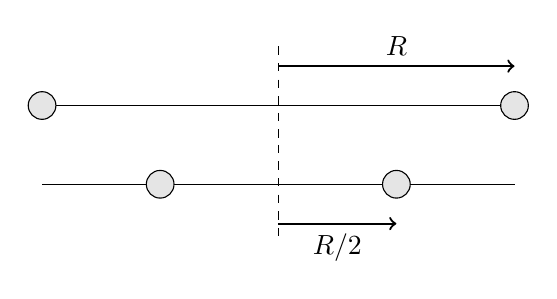
\begin{tikzpicture}
        \begin{scope}[yshift=+0.5cm]
            \draw (-3,0) -- (3,0);
            \draw[fill=white!90!black] (-3,0) circle (5pt);
            \draw[fill=white!90!black] (+3,0) circle (5pt);
            \draw[thick,->] (0,0.5) -- (3,0.5) node[pos=0.5,anchor=south] {$R$};
            \draw[dashed] (0,0.75) -- (0,-0.5);
        \end{scope}
        \begin{scope}[yshift=-0.5cm]
            \draw (-3,0) -- (3,0);
            \draw[fill=white!90!black] (-1.5,0) circle (5pt);
            \draw[fill=white!90!black] (+1.5,0) circle (5pt);
            \draw[thick,->] (0,-0.5) -- (1.5,-0.5) node[pos=0.5,anchor=north] {$R/2$};
            \draw[dashed] (0,0.5) -- (0,-0.75);
        \end{scope}
    \end{tikzpicture}
    \end{center}
    The system rotates at an angular velocity $\omega$ when the two masses $m$ are a distance $R$ from the axis.
    The masses are simultaneously pulled to a distance of $R/2$ from the axis by a force directed along the rod.
    What is the new angular velocity of the system?
    \begin{multicols}{3}
    \begin{choices}
        \wrongchoice{$\dfrac{\omega}{4}$}
        \wrongchoice{$\dfrac{\omega}{2}$}
        \wrongchoice{$\omega$}
        \wrongchoice{$2\omega$}
      \correctchoice{$4\omega$}
    \end{choices}
    \end{multicols}
\end{question}
}


%% PhysicsOlympiad 1996
%%----------------------------------------
\element{aapt}{ %% Olympiad-A6
\begin{question}{olympiad-1996-q13}
    A child with mass $m$ is standing at the edge of a playground merry-go-round with moment of inertia $I$,
        radius $R$, and initial angular velocity $\omega$.
    %% See figure to the right.
    \begin{center}
    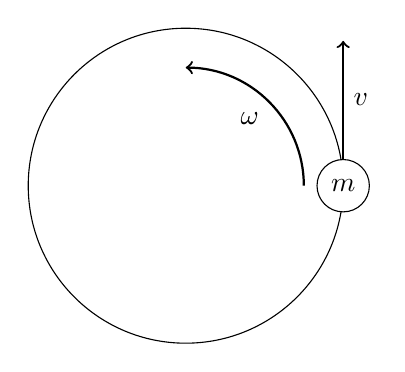
\begin{tikzpicture}
        \draw (0,0) circle (2cm);
        \node[draw,circle,fill=white] (M) at (2,0) {$m$};
        \draw[thick,->] (1.5,0) arc(0:90:1.5) node[pos=0.5,anchor=north east] {$\omega$};
        \draw[thick,->] (M.north) -- ++(90:1.5) node[pos=0.5,anchor=west] {$v$};
    \end{tikzpicture}
    \end{center}
    The child jumps off the edge of the merry-go-round with tangential velocity $v$ with respect to the ground.
    The new angular velocity of the merry-go-round is:
    %\begin{multicols}{2}
    \begin{choices}
        \wrongchoice{$\omega$}
        \wrongchoice{$\sqrt{\dfrac{I\omega^2 - mv^2}{I}}$}
        \wrongchoice{$\sqrt{\dfrac{\left(I+mR^2\right)\omega^2 - mv^2}{I}}$}
        \wrongchoice{$\dfrac{I\omega - mvR}{I}$}
      \correctchoice{$\dfrac{\left(I+mR^2\right)\omega^2 - mvR}{I}$}
    \end{choices}
    %\end{multicols}
\end{question}
}

\element{aapt}{ %% Olympiad-A6
\begin{question}{olympiad-1996-q14}
    As shown in the figure below,
        a spool has outer radius $R$ and axle radius $r$.
    A string is wrapped around the axle of the spool and can be pulled in any of the directions labeled by I, II, or III.
    \begin{center}
    \begin{tikzpicture}
        %% ground
        \draw (-2,0) -- (4,0);
        \node[anchor=north,fill,pattern=north east lines,minimum width=6.0cm, minimum height=0.05cm] at (1,0) {};
        %% spool
        \draw[thick] (0,2) circle (1cm);
        \draw[thick] (0,2) circle (2cm);
        \draw[thick] (0,0) -- (0,2);
        %% r and R
        \draw[thick,->] (0,2)-- ++(180:1) node[pos=0.50,anchor=south] {$r$};
        \draw[thick,->] (0,2)-- ++(215:2) node[pos=0.75,anchor=south] {$R$};
        %% I, II, and III
        %% NOTE: TODO: double check these angles
        \draw[thick,->] (0,2) ++(300:1) -- ++(30:2.2) node[anchor=south west] {III};
        \draw[thick,->] (0,2) ++(315:1) -- ++(45:2.2) node[anchor=south west] {II};
        \draw[thick,->] (0,2) ++(350:1) -- ++(80:2.2) node[anchor=south west] {I};
    \end{tikzpicture}
    \end{center}
    The spool will slide to the right without rolling on the horizontal surface if it is pulled in direction(s):
    \begin{multicols}{2}
    \begin{choices}
        %% NOTE: questionmult
        \wrongchoice{I only}
      \correctchoice{II only}
        \wrongchoice{III only}
        \wrongchoice{I and II only}
        \wrongchoice{II and III only}
    \end{choices}
    \end{multicols}
\end{question}
}

\element{aapt}{ %% Olympiad-A6
\begin{question}{olympiad-1996-q15}
    A uniform flag pole of length $L$ and mass $M$ is pivoted on the ground with a frictionless hinge.
    The flag pole makes an angle $\theta$ with the horizontal.
    The moment of inertia of the flag pole about one end is $\frac{1}{3} ML^2$.
    \begin{center}
    \begin{tikzpicture}
        %% ground
        \draw (-1,0) -- (5,0);
        \node[anchor=north,fill,pattern=north east lines,minimum width=6.0cm, minimum height=0.05cm] at (2,0) {};
        %% pivot and bar
        \draw (0,0) arc (270:-90:0.1cm);
        \draw[fill=white!90!black,rotate around={-45:(0,0.1)}] (-0.1,0.2) rectangle (0.1,5);
        \node[anchor=south west] at (45:5.0) {$P$};
        \draw[thick,<->] (-0.1,0.1) ++(135:0.5) -- ++(45:5) node[pos=0.5,anchor=center,fill=white,rotate=45] {$L$};
        %% angle
        \draw[<->] (1.5,0) arc(0:45:1.4) node[pos=0.5,anchor=west] {$\theta$};
    \end{tikzpicture}
    \end{center}
    If it starts falling from the position shown in the accompanying figure,
        the linear acceleration of the free end of the flag pole---labeled $P$---would be:
    \begin{multicols}{3}
    \begin{choices}
        \wrongchoice{$\dfrac{2g}{3}\cos\theta$}
        \wrongchoice{$\dfrac{2g}{3}$}
        \wrongchoice{$g$}
      \correctchoice{$\dfrac{3g}{2}\cos\theta$}
        \wrongchoice{$\dfrac{3g}{2}$}
    \end{choices}
    \end{multicols}
\end{question}
}


%% PhysicsOlympiad 1995
%%----------------------------------------
\element{aapt}{ %% Olympiad-A6
\begin{question}{olympiad-1995-q12}
    A solid cylinder weighing \SI{200}{\newton} has a fixed axis and a string wrapped around it.
    The string is pulled with a force equal to the weight of the cylinder.
    The acceleration of the string is approximately:
    \begin{multicols}{3}
    \begin{choices}
        \wrongchoice{\SI{10}{\meter\per\second\squared}}
      \correctchoice{\SI{20}{\meter\per\second\squared}}
        \wrongchoice{\SI{30}{\meter\per\second\squared}}
        \wrongchoice{\SI{40}{\meter\per\second\squared}}
        \wrongchoice{\SI{50}{\meter\per\second\squared}}
    \end{choices}
    \end{multicols}
\end{question}
}

\element{aapt}{ %% Olympiad-A6
\begin{question}{olympiad-1995-q13}
    A spinning ice skater has an initial kinetic energy $\frac{1}{2}I\omega^2$.
    She pulls in her outstretched arms,
        decreasing her moment of inertia to $\frac{1}{4}I$.
    Her new angular speed is:
    \begin{multicols}{3}
    \begin{choices}
        \wrongchoice{$\dfrac{1}{4}\omega$}
        \wrongchoice{$\dfrac{1}{2}\omega$}
        \wrongchoice{$\omega$}
        \wrongchoice{$2\omega$}
      \correctchoice{$4\omega$}
    \end{choices}
    \end{multicols}
\end{question}
}

\element{aapt}{ %% Olympiad-A6
\begin{question}{olympiad-1995-q14}
    A heavy rod of length $L$ and weight $W$ is suspended horizontally by two vertical ropes as shown below. The first rope is attached to the left end of the rod while the second rope is attached a distance $\frac{1}{4}L$ from the right end.
    \begin{center}
    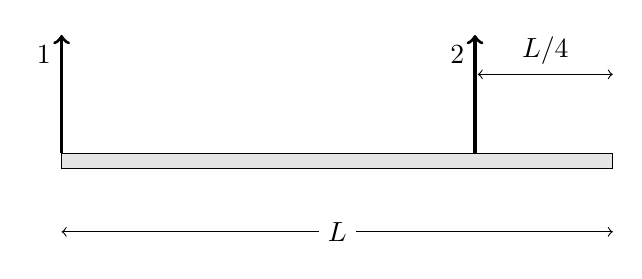
\begin{tikzpicture}[xscale=1.75]
        %% heavy rod
        \draw[fill=white!90!black] (-2,0) rectangle (2,-0.2);
        %% ropes
        \draw[very thick,->] (-2,0) -- ++(90:1.5) node[anchor=north east] {1};
        \draw[very thick,->] (+1,0) -- ++(90:1.5) node[anchor=north east] {2};
        %% labels
        \draw[<->] (-2,-1) -- (2,-1) node[pos=0.5,anchor=center,fill=white] {$L$};
        \draw[<->] (2,1) -- (1.02,1) node[pos=0.5,anchor=south] {$L/4$};
    \end{tikzpicture}
    \end{center}
    The tension in the second rope is:
    \begin{multicols}{3}
    \begin{choices}
        \wrongchoice{$\dfrac{1}{2}W$}
        \wrongchoice{$\dfrac{1}{4}W$}
        \wrongchoice{$\dfrac{1}{3}W$}
        \wrongchoice{$\dfrac{2}{3}W$}
        \wrongchoice{$W$}
    \end{choices}
    \end{multicols}
\end{question}
}


%% PhysicsOlympiad 1994
%%----------------------------------------
\element{aapt}{ %% Olympiad-A6
\begin{question}{olympiad-1994-q05}
    A top is spinning in the direction shown in the accompanying figure.
    \begin{center}
    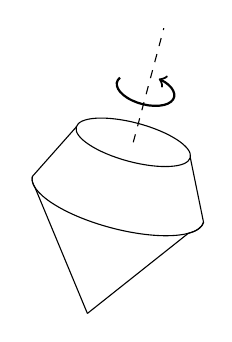
\begin{tikzpicture}
    \begin{scope}[rotate=-15,scale=0.75]
        %% top
        \draw (0,0) circle (1cm and 0.33cm);
        \draw (-1.5,-1) arc(180:360:1.5cm and 0.495cm);
        %\draw (0,-3) -- ++(130:2.0);
        \draw (-1,0) -- (-1.5,-1) arc(180:200:1.5cm and 0.495cm) -- (0,-3);
        \draw (+1,0) -- (+1.5,-1) arc(360:330:1.5cm and 0.495cm) -- (0,-3);
        %% spinning
        \draw[thick,->] (-0.5,1) arc (-200:70:0.5cm and 0.25cm);
        %% Axis
        \draw[dashed] (0,0) -- (0,2);
    \end{scope}
    \end{tikzpicture}
    \end{center}
    Its axis of rotation makes an angle of \ang{15} with the vertical.
    Assume friction can be neglected.
    The magnitude of the top's angular momentum will \rule[-0.1pt]{4em}{0.1pt} while its direction will \rule[-0.1pt]{4em}{0.1pt}.
    \begin{choices}
        \wrongchoice{increase; precess in the counterclockwise direction when seen from above.}
        \wrongchoice{increase; not precess}
        \wrongchoice{remain the same; not precess}
        \wrongchoice{remain the same; precess in the clockwise direction when seen from above.}
      \correctchoice{remain the same; precess in the counterclockwise direction when seen from above.}
    \end{choices}
\end{question}
}

\element{aapt}{ %% Olympiad-A6
\begin{question}{olympiad-1994-q10}
    A child of mass $M$ stands on the edge of a merry-go-round of radius $R$ and moment of inertia $I$.
    Both the merry-go-round and child are initially at rest.
    The child walks around the circumference with speed $v$ with respect to the ground.
    What is the magnitude of the angular velocity of the merry-go-round with respect to the ground?
    \begin{multicols}{2}
    \begin{choices}
      \correctchoice{zero}
        \wrongchoice{$\omega = \dfrac{MRv}{I}$}
        \wrongchoice{$\omega = \dfrac{v}{R}$}
        \wrongchoice{$\omega = \dfrac{MRv}{I-MR^2}$}
        \wrongchoice{$\omega = \dfrac{MRv}{I+MR^2}$}
    \end{choices}
    \end{multicols}
\end{question}
}

\element{aapt}{ %% Olympiad-A6
\begin{question}{olympiad-1994-q11}
    A rigid rod of mass $M$ and length $L$ has moment of inertia $\frac{1}{12} ML^2$ about its center of mass.
    A sphere of mass $m$ and radius $R$ has moment of inertia $\frac{2}{5} MR^2$ about its center of mass.
    A combined system is formed by centering the sphere at one end of the rod and placing an axis at the other (see accompanying figure).
    \begin{center}
    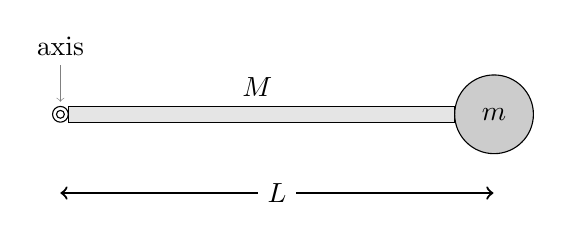
\begin{tikzpicture}
        %% Pivot Point
        \draw (0,0) circle (0.05cm);
        \draw (0,0) circle (0.1cm);
        \node[pin={[pin distance=5mm,pin edge={<-,shorten <=1pt}]90:axis}] at (0,0) {};
        %% Rod
        \draw[fill=white!90!black] (0.1,0.1) rectangle (5,-0.1);
        \node[anchor=south] at (2.5,0.1) {$M$};
        \draw[thick,<->] (0,-1) -- (5.5,-1) node[pos=0.5,anchor=center,fill=white] {$L$};
        %% Ball
        \node[draw,fill=white!80!black,circle,anchor=west,minimum size=1cm] at (5,0) {$m$};
    \end{tikzpicture}
    \end{center}
    What is the moment of inertia of the combined system about the axis shown?
    \begin{choices}
        \wrongchoice{$I = \dfrac{1}{12} ML^2 + \dfrac{2}{5} MR^2$}
        \wrongchoice{$I = \dfrac{1}{12} ML^2 + \dfrac{2}{5} MR^2 + mL^2$}
      \correctchoice{$I = \dfrac{1}{3} ML^2 + \dfrac{2}{5} MR^2 + mL^2$}
        \wrongchoice{$I = \dfrac{1}{12} ML^2 + mL^2$}
        \wrongchoice{$I = \dfrac{1}{3} ML^2 + mL^2$}
    \end{choices}
\end{question}
}

\element{aapt}{ %% Olympiad-A6
\begin{question}{olympiad-1994-q13}
    A uniform rod of length $L$ and weight $W_R$ is suspended as shown in the accompanying figure.
    \begin{center}
    \begin{tikzpicture}
        %% and wall
        \draw[thick] (0,-1) -- (0,6);
        \node[anchor=east,fill,pattern=north east lines,minimum width=0.1cm, minimum height=7cm] at (0,2.5) {};
        %% hinge and rod
        \draw (0.1,0) circle (0.1);
        \draw[fill=white!90!black] (0.2,-0.1) rectangle (6,0.1);
        \draw[very thick,->] (6,0.1) -- (6,-2) node[anchor=south east] {$W$};
        %% Cable
        \draw (6,0.1) -- (0,5);
        \draw[very thick,->] (6,0.1) -- ++(140.76:2) node[anchor=south west] {$T$};
    \end{tikzpicture}
    \end{center}
    A weight $W$ is added to the end of the rod.
    The support wire is at an angle $\theta$ to the rod.
    What is the tension $T$ in the wire?
    \begin{multicols}{2}
    \begin{choices}
        \wrongchoice{$T = \dfrac{W}{\sin\theta}$}
        \wrongchoice{$T = W + W_R$}
        \wrongchoice{$T = W + \dfrac{1}{2}W_R$}
      \correctchoice{$T = \dfrac{W + \dfrac{1}{2}W_R}{\sin\theta}$}
        \wrongchoice{$T = \dfrac{W + W_R}{\sin\theta}$}
    \end{choices}
    \end{multicols}
\end{question}
}

\element{aapt}{ %% Olympiad-A6
\begin{question}{olympiad-1994-q14}
    A hollow vertical cylinder of radius $R$ is rotated with angular velocity $\omega$ about an axis through its center.
    \begin{center}
    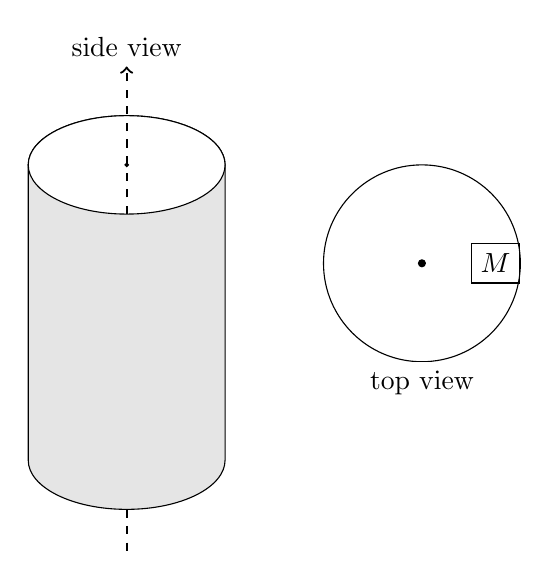
\begin{tikzpicture}[scale=1.25]
        \begin{scope}[xshift=-1.5cm]
            \draw[fill=white!90!black] (-1,0) arc (180:0:1cm and 0.5cm) -- (1,-3) arc(0:-180:1cm and 0.5cm) -- (-1,0) --cycle;
            %\draw[fill=white!50!black] (-1,0) arc(180:-180:1cm and 0.5cm);
            \draw[fill=white] (-1,0) arc(180:-180:1cm and 0.5cm);
            \draw[fill] (0,0) circle (0.5pt);
            \draw[thick,dashed] (0,-3.5) -- (0,-4);
            \draw[thick,dashed,->] (0,-0.5) -- (0,1) node[anchor=south,text width=5em,text centered] {side view};
        \end{scope}
        \begin{scope}[xshift=+1.5cm,yshift=-1cm]
            %\draw[fill=white!50!black] (0,0) circle (1cm);
            \draw[fill=white] (0,0) circle (1cm);
            \draw[fill] (0,0) circle (1pt);
            \node[anchor=north,fill=white] at (0,-1) {top view};
            \node[draw,minimum size=0.5cm,anchor=east] at (1,0) {$M$};
        \end{scope}
    \end{tikzpicture}
    \end{center}
    What is the minimum coefficient of static friction necessary to keep the mass $M$ suspended on the inside of the cylinder as it rotates?
    \begin{multicols}{2}
    \begin{choices}
        \wrongchoice{$\mu = \dfrac{gR}{\omega^2}$}
        \wrongchoice{$\mu = \dfrac{\omega^2 g}{R}$}
        \wrongchoice{$\mu = \dfrac{\omega^2 R}{g}$}
        \wrongchoice{$\mu = \dfrac{\omega^2}{gR}$}
      \correctchoice{$\mu = \dfrac{g}{\omega^2 R}$}
    \end{choices}
    \end{multicols}
\end{question}
}


\endinput


